              
%%%%%%%%%%%%%%%%%%%%%%%%%%%%%%%%%%%%%%%%%
% University Assignment Title Page 
% LaTeX Template
% Version 1.0 (27/12/12)
%
% This template has been downloaded from:
% http://www.LaTeXTemplates.com
%
% Original author:
% WikiBooks (http://en.wikibooks.org/wiki/LaTeX/Title_Creation)
%
% License:
% CC BY-NC-SA 3.0 (http://creativecommons.org/licenses/by-nc-sa/3.0/)
% 
% Instructions for using this template:
% This title page is capable of being compiled as is. This is not useful for 
% including it in another document. To do this, you have two options: 
%
% 1) Copy/paste everything between \begin{document} and \end{document} 
% starting at \begin{titlepage} and paste this into another LaTeX file where you 
% want your title page.
% OR
% 2) Remove everything outside the \begin{titlepage} and \end{titlepage} and 
% move this file to the same directory as the LaTeX file you wish to add it to. 
% Then add \input{./title_page_1.tex} to your LaTeX file where you want your
% title page.
%
%%%%%%%%%%%%%%%%%%%%%%%%%%%%%%%%%%%%%%%%%
\title{Uma introdução a Computação de Alto Desempenho}
%----------------------------------------------------------------------------------------
%   PACKAGES AND OTHER DOCUMENT CONFIGURATIONS
%----------------------------------------------------------------------------------------

\documentclass[12pt, a4paper]{report}
% Importando pacotes básicos
% Codificação
\usepackage[utf8]{inputenc}
% Linguagem
\usepackage[brazil]{babel}
% Fonte
\usepackage[T1]{fontenc}
% Determinando as margens do documento
\usepackage[left=3cm, right=2cm, bottom=2cm, top=3cm]{geometry}
% Possibilita o uso de LINKs e URLs ao longo do documento
\usepackage[pdftex, hidelinks]{hyperref}
% possibilita o uso do simbolo de graus 
\usepackage{gensymb}

% Pacotes que não lembro a funcionalidade
\usepackage{setspace}
\usepackage{graphicx} % Uso de figuras (ACHO)
\usepackage{float}
\usepackage{mathptmx}
\usepackage{amsmath}

% Permitir quebra de página nos ambientes de equações
\allowdisplaybreaks

% Acho que usei isso para colocar figuras em tabelas
\usepackage{subfig}

% Anexar PDFs no LaTeX
\usepackage[final]{pdfpages}

% Para colocar apêndices no LaTeX
\usepackage[toc,page]{appendix}

% Insercao de codigos no LaTeX
\usepackage{listings}
\lstset{language=Python}    % Setando a linguagem padrao

\usepackage{color}

\definecolor{codegreen}{rgb}{0,0.6,0}
\definecolor{codegray}{rgb}{0.5,0.5,0.5}
\definecolor{codepurple}{rgb}{0.58,0,0.82}
\definecolor{backcolour}{rgb}{0.95,0.95,0.92}

% Definindo estilo de exibição de código
\lstdefinestyle{mystyle}{
	backgroundcolor=\color{backcolour},   
	commentstyle=\color{codegreen},
	keywordstyle=\color{magenta},
	numberstyle=\tiny\color{codegray},
	stringstyle=\color{codepurple},
	basicstyle=\footnotesize,
	breakatwhitespace=false,         
	breaklines=true,                 
	captionpos=b,                    
	keepspaces=true,                 
	numbers=left,                    
	numbersep=5pt,                  
	showspaces=false,                
	showstringspaces=false,
	showtabs=false,                  
	tabsize=4,
	basicstyle=\scriptsize
}

% Para adicionar notas e TODO's
\usepackage{todonotes}

% Para colocar margem da na legenda de um figure/table
% \usepackage[margincaption,outercaption,ragged,wide]{sidecap}
% \sidecaptionvpos{figure}{t} 
\usepackage[figurename=Fig.]{caption}
\DeclareCaptionStyle{figstyle}
  [format=plain,margin=0pt,justification=centering]
  {format=hang,calcmargin={0pt,\widthof{\captionfont\captionlabelfont\figurename~\thefigure: }},
   font=small,labelfont=bf}
\captionsetup[figure]{style=figstyle}

% Indenta o primeiro parágrafo das seções
\usepackage{indentfirst}

% Pacote para o uso do biblatex como bibliografia
\usepackage[
    backend=biber,
    style=alphabetic,
    sorting=ynt
]{biblatex}
% Definindo o arquivo .bib de bibliografia
\addbibresource{BIB.bib}

% Translating mathematical function names to Portuguese
\let\sin\relax        \DeclareMathOperator{\sin}{sen}
\let\arcsin\relax     \DeclareMathOperator{\arcsin}{arcsen}

\begin{document}

	\begin{titlepage}
	
	\newcommand{\HRule}{\rule{\linewidth}{0.5mm}} % Defines a new command for the horizontal lines, change thickness here
	
	\center % Center everything on the page
	 
	%----------------------------------------------------------------------------------------
	%   HEADING SECTIONS
	%----------------------------------------------------------------------------------------
	
	\textsc{\LARGE Centro Federal de Educação Tecnológica de Minas Gerais}\\[3.5cm] % Name of your university/college
	\textsc{\Large Engenharia de Computação}\\[3.5cm] % Major heading such as course name
	
	%----------------------------------------------------------------------------------------
	%   TITLE SECTION
	%----------------------------------------------------------------------------------------
	
	\HRule \\[0.4cm]
	{ \huge \bfseries Paralelização de Métodos Numéricos para Resolver 
	Equações Diferenciais Parciais}\\[0.2cm] % Title of your document
	\HRule \\[2.5cm]
	 
	%----------------------------------------------------------------------------------------
	%   AUTHOR SECTION
	%----------------------------------------------------------------------------------------
	
	\begin{minipage}{0.4\textwidth}
	\begin{flushleft} \large
	\emph{Orientando:}\\ Marcelo Lopes de Macedo \textsc{Ferreira Cândido} % Your name
	\end{flushleft}
	\end{minipage}
	~
	\begin{minipage}{0.4\textwidth}
	\begin{flushright} \large
	\emph{Orientador:} \\
	Prof. Dr. Luis Alberto \textsc{D'Afonseca} % Supervisor's Name
	\end{flushright}
	\end{minipage}\\[7cm]
	
	% If you don't want a supervisor, uncomment the two lines below and remove the section above
	%\Large \emph{Author:}\\
	%John \textsc{Smith}\\[3cm] % Your name
	
	%----------------------------------------------------------------------------------------
	%   DATE SECTION
	%----------------------------------------------------------------------------------------
	
	{\large BELO HORIZONTE\\\today}\\[1cm] % Date, change the \today to a set date if you want to be precise
	
	%----------------------------------------------------------------------------------------
	%   LOGO SECTION
	%----------------------------------------------------------------------------------------
	
	%\includegraphics{logo.png}\\[1cm] % Include a department/university logo - this will require the graphicx package
	 
	%----------------------------------------------------------------------------------------
	
	\vfill % Fill the rest of the page with whitespace
	
	\end{titlepage}

    \lstset{style=mystyle}

    \tableofcontents
    
    \chapter{Introdução}

    \label{chp1}

    
    \chapter{Aquisições Sísmicas}

    \label{chp2}
    
    Nesse capítulo, serão explicados o que são aquisições sísmicas e 
    algumas formas pelas quais elas são realizadas. Além disso, se 
    mostrará o instrumento matemático pelo qual se pode modelar as 
    ondas sonoras (equação da onda) utilizadas nas aquisições 
    sísmicas e, por fim, um método para resolver tal instrumento 
    numericamente.

    \section{O Que São Aquisições Sísmicas e Como Modelá-las}

	No ramo da mineração não se pode tentar a esmo a descoberta de recursos
	minerais no subterrâneo de um local em que se já se suspeita sua existência.
	É necessário que, de alguma forma, se obtenha a forma dessa estrutura oculta
	para se saber os pontos onde se encontram as jazidas/poços desse recurso.
	A obtenção dos dados de como é essa estrutura se chama \textbf{aquisição
	sísmica}.

	A forma de se realizar essa aquisição pode variar com o ambiente, a coleta
	de dados e o método de processamento dos mesmos	adotado. Os recursos
	minerais desejados podem se encontrar tanto em meios terrestres e/ou
	subaquáticos. Contudo, o meio em que a aquisição será realizada pouco
	importa nesse trabalho, o que será melhor explicado mais a
	frente. Quanto aos métodos de processamento utilizados, apenas um nos
	importa: omodelamento da propagação de ondas, através dos meios (nesse caso,
	não homogêneos) nos quais se deseja realizar a aquisição, por um método
	matemático específico. Nesse trabalho, o método matemático aplicado, como já
	dito no Capítulo \ref{chp1}, é o de Diferenças Finitas.

	Já para a coleta dos dados a serem processados podemos citar dois exemplos
	de aquisição
	\begin{enumerate}
		\todo[inline]{buscar referências}
		\item \textbf{marítima}: um navio equipado com um canhão
		sonoro emite ondas sonoras cujas reflexões nas camadas terrestres
		submarinas são captadas por filas de geofones puxadas pelo mesmo navio.

		\item \textbf{terrestre}: um explosivo é colocado (preferencialmente
		enterrado) em um terreno. Sua explosão gera uma onda sonora cujas
		reflexões são 
	\end{enumerate}


    \section{A Equação da Onda}

Para que seja possível avaliar matematicamente um fenômeno ondulatório
produzido por uma fonte em um domínio é necessário se ter uma fórmula
matemática para o que se entende por onda. Tal fórmula, que nos servirá
durante todo esse trabalho (principalmente na parte da implementação
computacional) é a \textbf{equação da onda}, dada por
\begin{equation}
	\label{eq:waveEq}
	% dtt = 1 / v^2 (dxx + dyy) + f(x, y, t)
	\dfrac{\partial^2 u}{\partial t^2} =
	\dfrac{1}{v^2}
	\left(\dfrac{\partial^2 u}{\partial x^2} +
	\dfrac{\partial^2 u}{\partial y^2}\right) + f(x, y, t)
\end{equation}
onde $x$ e $y$ são variáveis espaciais e $t$, temporal. A constante $v$
representa (no caso desse trabalho) a velocidade da frente de onda. Trata-se de uma
\textbf{equação diferencial parcial hiperbólica} com solução analítica para alguns casos, mas
que pode ser resolvida numericamente, utilizando, por exemplo, o
Método de Diferenças Finitas, a ser discernido na próxima seção.

Caso o leitor se interesse por estudar ou revisar mais sobre Ondulatória, pode
conferir em Cândido \cite{mfcandido2018}.


    \section{O Método de Diferenças Finitas (MDF)}

	Uma equação diferencial parcial, que geralmente é considerada em um domínio 
	contínuo, pode ser discretizada. Isso é feito para que a equação possa ser 
	representada e resolvida computacionalmente. 
	
	No caso do método de diferenças	finitas para esse trabalho, basta 
	transcrever cada termo da equação para o equivalente na fórmula de 
	diferenças finitas para derivações de segundo grau, que é
	\begin{table}[H]
		\centering
		\begin{tabular}{c|c}
			\hline
			$\dfrac{\partial^2 u}{\partial x^2}$ & $\dfrac{u_{i-1} - 2u_i + u_{i+1}}{2\Delta x^2}$ \\ \hline
		\end{tabular}
	\end{table}
	


	
	    
\chapter{A arquitetura computacional atual e a necessidade de paralelização}

    Para compreender a questão da paralelização envolvida nesse trabalho é 
    necessário entender de onde e porque ela veio. Para tal, é necessário 
    se apresentar as principais peças que constituem um computador moderno, 
    os problemas que surgiram no processo de evolução da \textit{arquitetura 
    computacional} \todo{conferir se deve tratar como atual} atual e como isso culminou no paralelismo \cite{LLNL:parcomp}.

    Antes de iniciar esse processo, é também necessário se explicar o que se 
    entende por arquitetura computacional. Trata-se da área do conhecimento 
    que estuda a interface entre \textit{software} e \textit{hardware}, desde 
    o mais baixo nível, no qual o processador manipula as informações 
    (instruções e dados) entregues a ele, para toda operação realizada no 
    computador; passando pelas políticas de manipulação de dados nas memórias 
    cache (e seus níveis), de acesso aleatório (RAM - \textit{random access 
    memory}) e de armazenamento não-volátil (discos rígidos, por exemplo); 
    chegando também à interação dos computadores com os demais periféricos que 
    por ventura estão nele conectados, realizando \textit{inputs} (entradas) 
    e/ou \textit{outputs} (saídas), também conhecidas pela abreviação "I/O", 
    como teclado, \textit{mouse}, monitor, etc \cite{Catsoulis}.
    
    Ainda no âmbito da arquitetura de computadores, são estabelecidas análises e 
    metas de performance. Por exemplo, tenta-se determinar se um processador A é 
    mais rápido que um B (sendo B diferente de A) comparando-se o número de 
    instruções que cada um processa, ou quantos ciclos (que serão explicados mais 
    a frente) podem ser dados em um segundo \cite{wiki:comparch}. 
    Questão semelhante encontra-se na 
    computação de alta performance\footnote{\textbf{computação de alta performance} 
    (ou \textbf{supercomputação}) é um ramo da computação que usa supercomputadores 
    e estuda técnicas de paralelismo visando alcançar velocidades de processamento 
    maiores (do que as de computadores normais, como os pessoais) para a resolução de 
    problemas computacionais complexos, como simulações, 
    modelagens e análises computacionais. Esse ramo também pode, no lugar de focar 
    em processamento mais rápido, resolver problemas de dimensões maiores, que não 
    poderiam ser resolvidos em tempo hábil por computadores comuns \cite{techo:hpc}}: 
    quão mais rápido um trecho de código executa ao ser paralelizado.
   
    Essa organização focada em um processador, memórias cache, RAM e de 
    armazenamento não-volátil vieram da \textbf{arquitetura de von Neumann}, 
    que possui esse nome por conta de seu idealizador, John von Neumann.

    \section{A arquitetura de von Neumann}
   
    \begin{itemize}
        \item von Neumann e o conceito de programa armazenado;
        \item a forma da arquitetura (componentes e ligações);
        \item o contraste da arquitetura idealizada com as anteriores.
    \end{itemize}
    
    \subsection{O gargalo de von Neumann}
    
        \begin{itemize}
            \item o gargalo existente entre o processador e a memória, 
            que não consegue acompanhá-lo.
        \end{itemize} 
	    
    \section{O Processador}

\label{sec:processor}

Um processador consiste em um módulo de \textit{hardware} capaz de manipular
\gls{instr-machine} armazenadas
em memória e produzir os resultados desejados através dessas instruções. Tais resultados
podem ser de cunho ou lógico-aritmético ou manipulação de dados, no geral. Tal módulo é
indispensável para o conceito de computadores como conhecemos hoje, de tal forma que, se
não fosse pela necessidade de memória para a armazenagem de dados, um processador poderia
ser a definição de um computador. Um exemplo de processador pode ser visualizado nas Figuras
\ref{subfig:processor-example-1} e \ref{subfig:processor-example-2}.

\begin{figure}[H]
    \centering
    \begin{subfigure}{.5\textwidth}
        \centering
        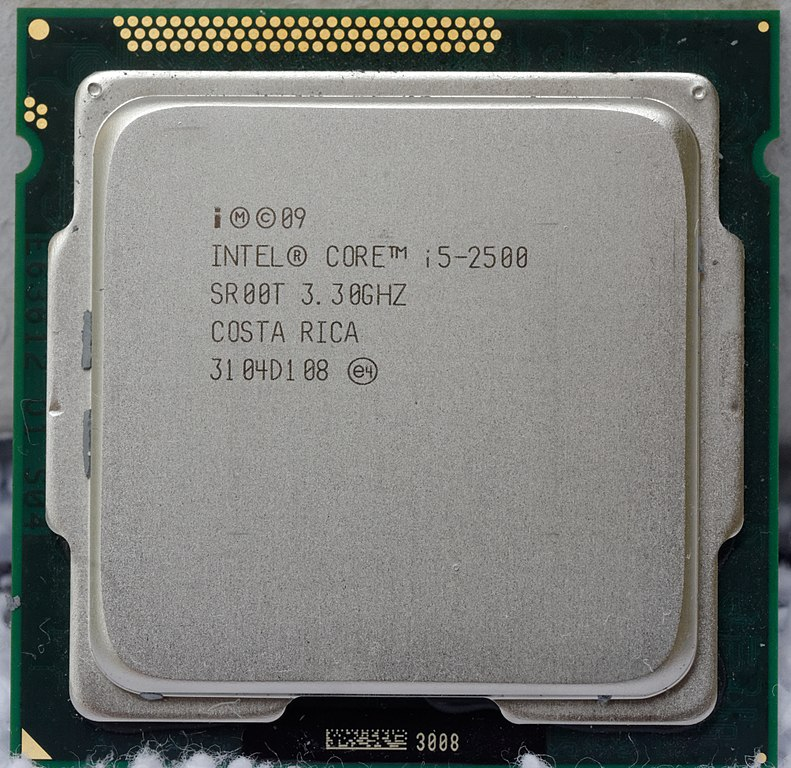
\includegraphics[width=.7\linewidth]{chapters/chp3/images/intel-i5-2500-processor.jpg}
        \caption{Um processador Intel\textsuperscript{\textregistered} 2500 \cite{wiki:i5_2500}.}
        \label{subfig:processor-example-1}
    \end{subfigure}
    \begin{subfigure}{.5\textwidth}
        \centering
        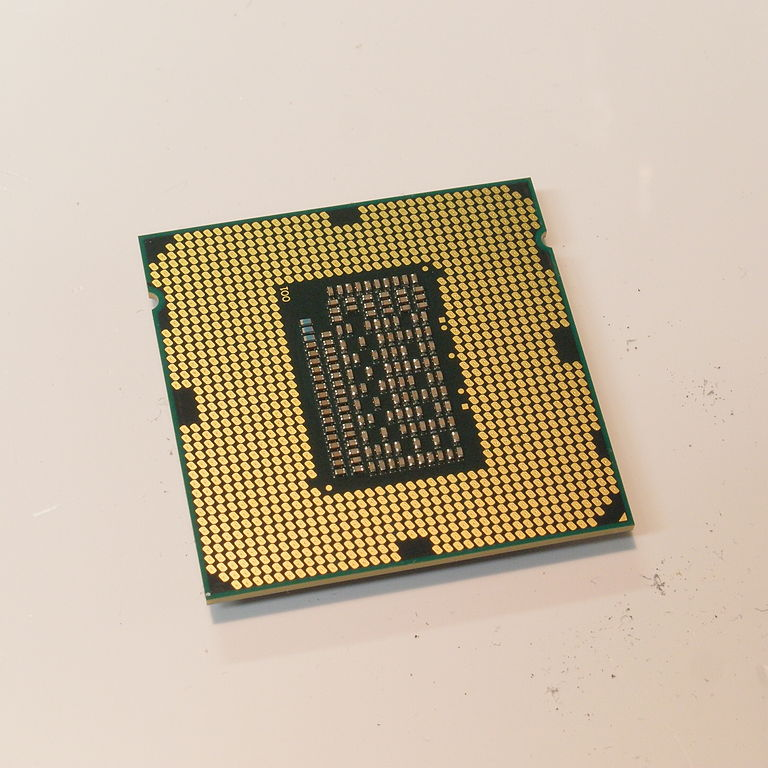
\includegraphics[width=.7\linewidth]{chapters/chp3/images/intel-i7-2600k-processor-pins.jpg}
        \caption{Os pinos de um processador Intel\textsuperscript{\textregistered} 2600 \cite{wiki:i7_2600}}
        \label{subfig:processor-example-2}
    \end{subfigure}
    \caption{Exemplos de processadores}
    \label{fig:processors}
\end{figure}
	    
    \section{A Memória Principal}

Quando se fala sobre memória computacional, pode-se estar referindo à memória 
cache, \acrfull{ROM}, \acrfull{RAM} ou à capacidade de armazenamento de um disco rígido. 
Dentre essas, a \acrshort{RAM} é considerada a principal e um exemplo dela 
pode ser visto na Figura \ref{fig:ram}. Ela é responsável por 
armazenar os programas em forma de processos gerenciados pelo sistema operacional, ou seja, 
enquanto eles estão sendo executados. Ela também é responsável por armazenar todos os dados 
gerados por um programa que ainda não foram ou descartados, ou salvos em disco ou cujo acesso 
ainda é requisitado.

Outras características sobre a \acrshort{RAM} são: 
\begin{itemize}
    \item o fato de que ela apenas armazena os dados até ser desligada, o que a classifica 
    como memória volátil;
    \item sua capacidade de armazenamento, que, na maioria dos casos, é maior do que a de memórias 
          cache e menor do que a de discos rígidos;
    \item sua velocidade, que segue o inverso da capacidade de armazenamento, ou seja, é menor do 
          que a de memórias cache e maior do que a de discos rígidos.
\end{itemize}

\begin{figure}[H]
    \centering
    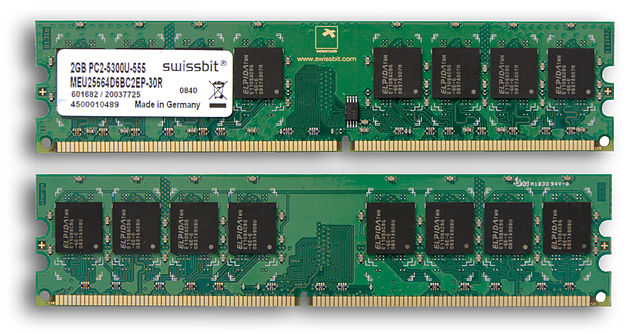
\includegraphics[scale=1.5]{chapters/chp3/images/Swissbit-2GB-PC2-5300U-555.jpg}
    \caption{Dois módulos de \acrshort{RAM} Swissbit\textsuperscript{\textregistered} 
    PC2-5300 DDR2 com capacidade de 2 Gigabytes, utilizada em computadores de mesa \cite{wiki:ddr2_ram}.}
    \label{fig:ram}
\end{figure}
	    
    \section{A cache}

    \begin{itemize}
        \item O princípio da localidade no tempo e no espaço;
        \item A necessidade da existência de uma cache, visto o 
        princípio da localidade;
        \item Explicação do que é uma cache;
    \end{itemize}
    
    \chapter{Disco rígido}

    \begin{itemize}
        \item O que são memórias voláteis e exemplos delas;
        \item A necessidade de memórias não-voláteis e o HD;
        \item Outras diferenças entre o HD e as outras memórias 
        envolvidas no trabalho
    \end{itemize}

	\section{Conseguir mais em menos tempo}

    \begin{itemize}
        \item A necessidade de se aumentar a velocidade de processamento;
        \item introdução aos problemas encontrados na computação serial
    \end{itemize}

    \subsection{A barreira da memória - \textit{Memory wall}}
    
        \todo[inline]{Conferir se existe mesmo a memory wall}
        \todo[inline]{Revisar o que é a memory wall e completar o itemize abaixo}
    
        \begin{itemize}
            \item 
        \end{itemize}
    
    \subsection{A barreira do paralelismo a nível de instruções - \textit{ILP wall}}
    
        \begin{itemize}
            \item Explicar do que se trata o paralelismo a nível de instruções;
            \item Explicar os conceitos de superpipeline e superescalar;
            \item Explicar que, ao se estender muito um pipeline, temos problemas;
            \item Explicar os problemas da superescalaridade
        \end{itemize}
    
    \subsection{A barreira no gasto de energia dos processadores - \textit{Power wall}}
    
        \begin{itemize}
            \item Introduzir a lei de Moore;
            \item Explicar que houve evolução na taxa de clock ao longo do tempo;
            \item Explicar que essa evolução foi amortecida nos últimos anos devido 
            ao gasto energético e às altas temperaturas que os processadores alcançaram 
        \end{itemize}
	
	\section{Paralelismo - a alternativa para se contornar as barreiras}

    \begin{itemize}
        \item Explicar no que consiste o paralelismo;
        \item em seguida, explicar porquê ele é uma saída possível
    \end{itemize}
    
    \subsection{Arquiteturas de memória na computação paralela}
    
        \begin{itemize}
            \item Explicar as arquiteturas:
            \begin{itemize}
                \item de memória compartilhada;
                \item memória distribuída;
                \item híbrida
            \end{itemize}
        \end{itemize}
    
    \subsection{Modelos da computação paralela}
    
        \todo[inline]{Conferir se serão esses modelos a serem apresentados}
    
        \begin{itemize}
            \item Shared Memory Model;
            \item Threads Model;
            \item Distributed Memory / Message Passing Model;
            \item Data Parallel Model;
            \item Hybrid Model
        \end{itemize}
    
    \subsection{Desenhando programas paralelos}
    
        \todo[inline]{ler a respectiva seção e completar aqui}
    
        \begin{itemize}
            \item 
        \end{itemize}
    
    \chapter{Paralelismo em prática}

Para facilitar o desenvolvimento de \textit{software} com paralelização, foram 
criadas interfaces com rotinas (funções) que servem de abstração para o desenvolvedor.
Dessa forma, este se preocupará apenas com as estratégias de paralelização a 
serem adotadas e não como o paralelismo deve ocorrer em \gls{low-level}. Tais interfaces 
são chamadas \acrfull{api} e são indispensáveis para esse trabalho.

Nesse capítulo serão abordadas as três \glspl{API} que foram utilizadas para a 
realização desse trabalho: \acrshort{openmp}, \acrshort{pthreads} e \acrshort{openmpi}.

\section{OpenMP}

\label{sec:openmp}

A \acrshort{api} \acrfull{openmp} consiste em rotinas, 
variáveis de ambiente e diretivas de compilação reunidas em um 
modelo portável e escalável que serve como uma interface para 
desenvolvedores criarem aplicações paralelas com simplicidade e 
flexibilidade \cite{wiki:openmp}. Essa \acrshort{api} se encontra 
incluída no modelo de computação paralela de memória compartilhada, 
assim como a \acrshort{pthreads}.

\subsection{Diretiva Utilizada}
\begin{lstlisting}
#pragma omp parallel for
\end{lstlisting}
Considerada uma diretiva de compartilhamento de trabalho, essa 
ferramenta permite que qualquer laço de repetição do tipo \texttt{for} 
(nas linguagens C/C++, 
\lstinline[columns=fixed]{for(int i = 0; i < ALGUM_NUMERO; i++)// faz algo}, 
por exemplo) tenha seu número de iterações dividido entre $n$ \textit{\gls{threads}}, 
sendo $0 < n <= \text{número máximo de threads}$.

\section{\texttt{Pthreads}}

\section{MPI}

	\begin{itemize}
		\item Do que se trata a MPI e onde ela está incluída;
		\item um programa hello world com MPI.
	\end{itemize}

    
    \chapter{Do serial ao paralelo}

\label{cap:implementation}

Como já dito anteriormente, o objetivo desse trabalho é a construção
de um código paralelizado capaz de resolver a equação da onda utilizando
o Método de Diferenças Finitas. O presente capítulo apresentará a
construção desse código, partindo do serial equivalente, passando pelos
estudos realizados com as \glspl{api} e concluindo com a construção do
código paralelo final.

\section{A Construção do Código Serial}

Como dito anteriormente na Seção Código \ref{subsec:parallel-design},
após se compreender o problema a ser programado em termos paralelos,
deve-se então criar o código serial que resolve o problema.

Para tal, criaram-se as \glspl{class} \texttt{\_2Dwave} (Código \ref{code:wave-serial}), que visa representar as características da
onda e também da sua fonte; \texttt{interface} (Código \ref{code:interface-serial}) e \texttt{velocity}
(Código \ref{code:velocidade-serial}), que buscam representar as características do meio em que a onda propagará.
Para unir essas informações e realizar os cálculos da propagação da onda utilizando o Método de Diferenças Finitas, foi
criado o programa principal (Código \ref{code:main-serial}).

\subsection{Camadas}
É importante relembrar que quando se fala de camadas se refere às porções de solo subterrâneas
que estão isoladas umas das outras por características diferentes e bem definidas (como o material
de que são feitas e o quanto esse está comprimido, por exemplo). Duas características do meio podem ser
usadas para a simulação da propagação das ondas: ângulo que as interfaces (limite de uma camada para a outra,
sendo representadas por funções de primeiro nesse projeto) possuem e a velocidade (representada por uma funcão de
primeiro grau com duas variáveis) das camadas.

\subsubsection{Interfaces}
Tanto no código serial quanto no final (paralelo), as interfaces das camadas são representadas
pela \gls{class} \texttt{interface}. Tal \gls{class} possui dois atributos: \texttt{a} (coeficiente angular) e
\texttt{b} (termo constante). Além disso, ela também possui um método, \texttt{getY(\textbf{double} x)}, responsável por retornar
o $y$ da reta para um dado $x$.

\subsubsection{Velocidades}
Já quanto às velocidades das camadas, no código serial e no final (paralelo), elas são representadas
pela \gls{class} \texttt{velocity}. Essa \gls{class} possui três atributos: \texttt{a}, \texttt{b} e \texttt{c},
sendo os dois primeiros os multiplicadores das variáveis $x$ e $y$ da função que representa a velocidade; e o último
sendo o termo constante. A \gls{class} também possui o método \texttt{getGradientVelocity(\textbf{double} x, \textbf{double} y)}
que retorna a velocidade encontrada em um determinado ponto $(x, y)$ da camada.

\subsection{Onda}
A onda bidimensional que será propagada através do meio é representada pela \gls{class} \texttt{\_2Dwave}, que possui como
atributos: a extensão do domínio em $x$ (\texttt{Lx}) e $y$ (\texttt{Ly}), o tempo máximo que a simulação
da propagação deve durar (\texttt{tMax}), número de pontos em $x$ (\texttt{Mx}) e $y$ (\texttt{Ny}), para
a discretização do domínio; a frequência da onda (\texttt{w}), sua amplitude (\texttt{A}), seu ponto $(x, y)$ e tempo iniciais
(\texttt{Xp}, \texttt{Yp} e \texttt{Tp}).

Além desses atributos, a \gls{class} também possui os métodos
\texttt{evaluateFXYT(\textbf{double} x, \textbf{double} y, \textbf{t})}, que retorna a amplitude da onda para determinado ponto
$(x, y, t)$; e \texttt{getVelocitiesMatrix(\textbf{vector<interface>} interfaces, \textbf{vector<velocity>} velocities)},
que retorna uma matriz da velocidade de cada ponto $(x, y)$ do domínio.

\subsection{O Programa Principal}
O programa principal consiste, basicamente, em recolher as informações dadas pelo usuário por meio do Código
\ref{code:cli-serial}; Em seguida, realizar os cálculos do Método de Diferenças Finitas e, por fim, salvar
os dados resultantes a esses cálculos, que podem ser matrizes, das quais se pode obter imagens da onda propagando; ou vetores, dos
quais se pode obter os traços sísmicos registrados pelos receptores simulados.

\subsection{Os Códigos Auxiliares ``Falsos''}
Também foram criados códigos seriais ``falsos'' para que a construção do código final acontecesse de forma mais gradual e didaticamente.
São chamados ``falsos'' porque buscam resolver problemas mais fáceis que o problema real que o projeto busca solucionar. Sobre
eles foram construídos níveis de paralelização como forma de estudo para que os níveis a serem implementadas no código real
fossem feitos mais facilmente.

O primeiro desses códigos (Código \ref{code:parabolloid-serial}) preenche uma matriz com os valores em $z$ do paraboloide $z = 2x^2 + y^2$,
sendo os limites de $x$ e $y$ delimitados pelo usuário. Já o segundo (Código \ref{code:fdm-1d-serial}) calcula a propagação de uma onda
unidimensional sobre uma corda ao longo do tempo, cujos limites também são definidos pelo usuário.

O primeiro código citado propõe a introdução facilitada de níveis de paralelização, não havendo nenhum problema que exija
um nível maior de atenção. Já o segundo, por conta de que os cálculos do próximo instante de tempo $t_1$ dependem de que os cálculos de $t_0$
(com $t_0 < t_1$) estejam finalizados, insere o problema da sincronização ao se aplicar paralelismo com \gls{threads}. Estudar esse problema
é essencial antes de se implementar o código final.



\section{Primeiro contato do código com as \textit{threads} - OpenMP}

    \subsection{Construindo o caminho para a OpenMP}
    
	    \begin{itemize}
	    	\item Explicar o código fake da avaliação de função;
	    	\item explicar o código fake das diferenças finitas 1D.
	    \end{itemize}

\section{Um contato mais profundo com as \textit{threads} - Pthreads}
Essa Seção visa apresentar os códigos ``falsos'' envolvendo a \acrshort{api} \acrfull{pthreads}.
O primeiro desses mostrará como dividir o trabalho da avaliação da função de um paraboloide 
entre \glspl{threads}. Já o segundo fará algo semelhante, mas considerando que o trabalho de todas as 
\glspl{threads} deve ter terminado para se iniciar a próxima iteração de cálculos. 

\subsection{Avaliação de uma função}
Para dividir o trabalho entre as \glspl{threads}, inseriu-se uma \gls{struct} no Código \ref{code:parabolloid-pthreads}, cuja as instâncias seriam dadas às \glspl{threads}, uma instância para cada. 
Nessa \gls{struct} existe um ponteiro para a matriz de cálculos, os limites desta determinados para cada \gls{threads}, os valores iniciais para esses limites e os valores de \textit{offset} para cada dimensão.

O funcionamento do Código se baseia na utilização da função \texttt{pthread\_create()} para lançar as \glspl{threads} que se utilizarão da função \texttt{calculate()} para executar os cálculos das suas respectivas porções da matriz. Existe também no Código a função \texttt{pthread\_join()}, que foi utilizada apenas para ilustração e, principalmente, treino para o assunto da próxima Seção.

\subsection{Propagação de onda em uma dimensão}
Possuindo uma estrutura semelhante ao código tratado pela Seção anterior, o Código \ref{code:fdm-1d-pthreads}, responsável por simular a propagação de uma onda unidimensional, possui como diferença essencial a necessidade de certificar que nenhuma outra \gls{threads} será criada antes que as atuais tenham terminado seu trabalho. 

Essa característica se deve ao fato de que não se pode calcular o próximo instante de tempo sem o anterior, visto como é definido o Método de Diferenças Finitas para a equação da onda. Dessa forma, o funcionamento da \texttt{phtread\_join()} se torna mais necessário com esse Código.

\section{Realizando a mescla de \texttt{Pthreads} e \texttt{MPI}}
    
    \subsection{Contruindo o caminho para a mescla}
    
    \chapter{Considerações finais}
    
    % Definindo o estilo de bibliografia
% 	\bibliographystyle{abbrv}

    % Printando a bibliografia
    \printbibliography
    
\end{document}